\startchapter{Single Hop Transmission}
\label{chapter:single}

This is chapter expalins the rss-grouping work.

There has been a massive increase in the number of nodes connected to an Access Point (AP) in a Wireless Local Area Network (WLAN) in recent years. Technologies such as Internet of Things (IoT), sensor networks and Machine Type Communication (MTC) are anticipated to bring an even larger number of nodes all contending to access the license-free Industrial, Scientific, and Medical (ISM) bandwidth. This is part of the reason that the next generation of IEEE 802.11 standards includes a new sub 1GHz bandwidth to ISM in order to cover the IoT traffic \cite{Req80211ah}. But the number of connections from both MTC and human devices increases so fast that using conventional IEEE 802.11 MAC protocol's Distributed Coordination Function (DCF) to handle such a large number of nodes results in a high collision probability and very low channel efficiency.

Research efforts have been put to make super dense IEEE 802.11 networks more efficient. In addition to physical layer solutions trying to make wireless communications more efficient and faster, a key issue is how to modify the DCF protocol in the MAC layer to achieve better resource utilization. For instance, \cite{zhong2014dcf} proposed a method to adjust the transmission opportunity according to collision probability. One promising solution is grouping users and limiting the competitions within the group, used in Group Synchronized Distributed Coordination Function in the IEEE 802.11ah standard \cite{Draft80211ah}. It has been proved in \cite{zheng2014performance} and \cite{raeesi2014performance} that grouping users and dedicating a Restricted Access Window (RAW) to each group increases the overall throughput in wireless networks. \iffalse CHECK THIS \fi The work at \cite{kim2015optimal} has also addressed the problem of super dense networks and proposed a grouping scheme based on transmission attempts to assign larger RAWs to crowder groups instead of having equally timed RAWs. 


\section{802.11ah Standrad}
 Explain what 802.11ah is.

 The 802.11ah protocol is one of the recent standards by IEEE organization. This standard introduces many new concepts for the first time, including new designs for both physical and MAC layer. The 802.11ah standard has been designed with three use cases in mind, smart sensors, back-haul aggregation and extended range hot-spot. In smart sensor use case, 802.11ah is designed to handle a very large number of nodes(up to 6000) connected to one access point. In the back-haul use case, an 802.11ah access point is designed to be used as an aggregator for wireless personal area network(WPAN) devices that use IEEE 802.15.4.g standard. WPAN(802.15.4g) devices have small transmission range and data rate, so in this case, 802.15.4g routers, gather data from 802.15.4g devices and send them to a single 802.11ah aggregator. In the extended hot-spot use case, 802.11ah access points can be used as cellular offloading candidates specially in outdoor environment where other .11 standards suffer from their short range.

\subsection{Physical Layer of 802.11ah}
In the Physical Layer(PHY), 802.11ah makes use of sub 1GHz license-exempt bands. This is the main physical layer difference between this standard and previous .11 standards. Also, 802.11ah mostly focuses on small bandwidths and does not allow >20 MHz bands. The use of smaller carrier frequency also gives 802.11ah a much larger transmission range compared to other .11 standards. In outdoor scenarios, using default transmission power(200mW), 1MHz channel and Modulation and Coding Scheme(MCS) 10, it can achieve a range as high as 1 km.   

\subsection{MAC layer of 802.11ah}
 In the MAC layer 802.11ah introduces may new concepts from frame formats to channel access and power management. In the main 802.11 standard, number of nodes that can be connected to one access point is limited to 2007. 802.11ah extends this range to 8191 nodes to support the smart sensor use case. Also to better support dense network scenarios, 802.11ah shortens the length of frame headers, control frames such as ACKs and periodically transmitted frames such as beacons. The main change in 802.11ah which is also the focus of this paper are changes in the channel access. 

 In order to handle the large contention between nodes in dense scenarios, 802.11ah divides all nodes connected the access point into different groups, each is then given a specified time window called Restricted Access Window(RAW) to use the channel while members of all other groups remain silent. This also divides the beacon period into multiple RAWs each dedicated to one group. This not only decreases the contention that one node experiences while using the wireless channel, also lets nodes save power by going to sleep in RAW that do not belong to them. It is left to the access point to decide whether or not  to allow nodes to cross the RAW boundary just to finish an ongoing transmission(Cross Slot Boundary). This channel access mechanism is called Group Synchronized Distributed Coordination Function (GS-DCF) which is to be used instead of the traditional DCF.   

\section{The Hidden Terminal Problem}

Explain what hidden terminal problem is.

The hidden terminal is a traditional problem in wireless communication. Is usually happens when a node falls outside of sensing area of another node but they are both trying to communicate with a same node. Figure \ref{fig:hidden} illustrates a general case for the hidden terminal problem. For example, if the node A, first start the transmission of a packet to node B, and sometime in the middle of their communication, node C also decides to transmit a packet to B, according to the CSMA/CA procedure it will first listen to the channel, an since it can not sense the transmission coming from A. it will find the channel ideal and initiate its transmission to B which will result in collision and loss of both packets of A and C. Wireless LAN in the infrastructure mode considering the up-link transmission, since every other node wants for transmit to the access point, are vulnerable to this problem. 


\begin{figure} [!tbp]
  \centering
  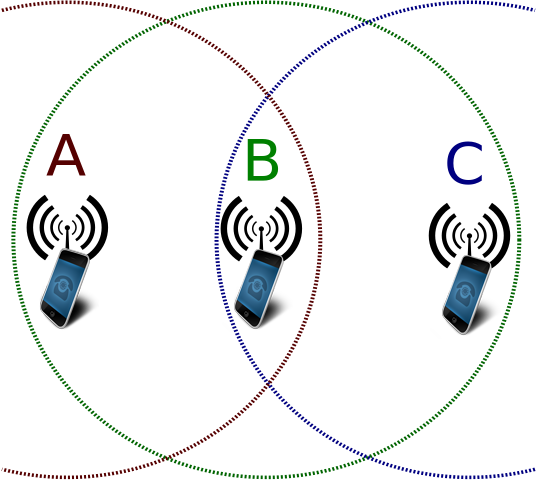
\includegraphics[width=.95\textwidth]{figures/hidden}
  \caption{A simple hidden terminal problem}
  \label{fig:hidden}
\end{figure}

The legacy solution for this problem is the use of Request To Send(RTS) and Clear To Send(CTS) messages. Using these messages, every node has to send an RTS to its receiver and wait to get a CTS before starting a transmission. In this way, although node C might not sense the RTS from node A, it will receive the CTS that B sends to A and know that the channel for B is going to be busy. The only chance of collision because of the hidden terminal then is during the transmission of the RTS message. Since the RTS is a small control message, collision probability will be reduced significantly. 

Given the extended range of communication in the 802.11ah standard, this problem becomes even more serious.  

\section{Related Works}

\cite{tsertou2008revisiting} has considered the hidden terminal with a new approach in a Constant Contention Window (CCW) scenario and studied the problem of two competing senders that cannot sense each other but are trying to transmit to a station that both can sense, a frequent situation in infrastructure mode networks.

One solution for the hidden terminal problem is using RTS/CTS mechanism. This mechanism solves the problem for the case that the transmission time of a data packet is much larger than that of RTS/CTS. However, it introduces additional overhead, and the collisions cannot be avoided due to the RTS packets from hidden terminals. In \cite{yoonregrouping}, the hidden terminal problem in GS-DCF based networks was discussed. The proposed hidden matrix based regrouping (HMR) algorithm can reduce the number of hidden terminals but it is a centralized approach and requires the access point to discover hidden terminal relationship between two nodes first and then solve it by regrouping one of them to another group.

The research in \cite{tseng2014effective} has also studied the hidden terminal problem but in IEEE 802.15.4-based networks. A grouping mechanism similar to IEEE 802.11ah is proposed but the strategy to deal with the hidden terminal problem is still based on discovering hidden terminal relationships and rescheduling nodes.

\cite{abichar2013group} proposed a Group-based MAC where a new station join a group if the estimated distance to the group leader is below half of the transmission distance to avoid hidden-terminal, and otherwise a new group will be formed. The AP cannot effectively control the number of groups.

%The optimum way to have location based groups and solve most of potential hidden terminal problems would be the case that access point knows location information of each node and uses a clustering algorithm such as K-Means to categorize nodes in different groups and then assign each node to its designated group in way similar to centralized grouping schemes described in \cite{zheng2014performance}. 
When the AP can obtain the global information about the location of all nodes, existing clustering algorithms such as k-means can be applied and the group designation is completely controlled by the AP in a way similar to centralized grouping schemes described in \cite{zheng2014performance}.

However, when the number of terminals is large, collecting global information significantly increases the overhead of feedback. Assigning all of the nodes to their groups results in a high control overhead especially when the network is dynamic.


\section{Rss-Based Grouping Strategy}

\subsection{Motivation}

Although using GS-DCF function proposed in IEEE 802.11ah can improve final throughput compared to conventional IEEE 802.11 protocols, there are still some open issues resulting from the new sub 1GHz license-exempt bands in IEEE 802.11ah. Utilizing carrier frequencies smaller than $1$ GHz can increase network coverage up to $1$ km. This large distance makes the well-known hidden terminal problem more serious. As shown in \iffalse CHECK THIS \fi \cite{wu2006wsn02,tsertou2008revisiting,khurana1999performance}, the hidden terminal problem can lead to a substantial performance degradation in infrastructure-based networks. 

Although RTS/CTS and centralized grouping strategy have been proposed to address the hidden terminal problem \cite{yoonregrouping,tseng2014effective}, they are not suitable for IoT scenarios with small packet size and large number of nodes.

 %\cite{tsertou2008revisiting} and \cite{khurana1999performance} have also suggested models which consider the hidden terminal and show the performance degradation. 

  Based on the grouping idea in the IEEE 802.11ah standard, this chapter aims to solve the problem in a distributed manner without using RTS/CTS. Our solution ensures that nodes in the same group are close enough to each other so that they can always sense each other's transmission in their own RAW. 

Different from the previous approaches, this thesis proposes an RSS-based grouping scheme.
Nodes sense the received power from other nodes and join the group that has the largest sensed power. To the best of our knowledge, this is the first work to explicitly use signal strength for assigning nodes to their groups. The performance gain of the proposed method is then evaluated by analytical model and simulations. \iffalse CHECK THIS \fi The main contributions of this paper are three-fold. First, we propose an RSS-based grouping strategy to solve the hidden terminal problem in IEEE 802.11ah networks. Second, we derive the probability of two nodes in one group being able to sense each other. Third, extensive simulations using NS-2\cite{breslau2000advances} have been conducted, and the results show that, by using the proposed method, the hidden terminal problem becomes negligible in IEEE 802.11ah networks and RTS/CTS is no longer needed.


\subsection{System Model} \label{systemmodel}

In this work, we consider an infrastructure based IEEE 802.11ah network, where each wireless terminal transmits its packets directly to the access point. %For simplicity, we only consider upload traffic from nodes to the access point, same as the in \cite{wu2006wsn02}. 
The network coverage area is a circle with radius $R$ where the access point is at the center. Nodes are uniformly distributed in the circle and their locations follow a Poisson Point Process (PPP) with density $\lambda$. The latter two assumptions are used for analysis and they are not necessary for the algorithm to perform. Nodes are assumed to be static at their position which is a reasonable assumption for most IoT and sensor networks and an active node always has a packet to transmit. %Active nodes are assumed to have saturated traffic. % which means every node has always a packet to transmit.

The channel model used in the analysis is a pathloss model with parameters $\alpha$ and $\beta$ in a way that the received power at a distance $d$ from the transmitter node is
\begin{equation}
P_r(d)=\frac{\beta}{d^\alpha} P_t,
\end{equation}
where $P_t$ is transmit power. In the simulation, we also consider the Rayleigh fast-fading and log-normal shadowing model where the received power is an exponential random variable and its mean $\bar{\gamma}$ is a log-normal random variable as 
\begin{equation}
\bar{\gamma}_{dB}= \mathcal{N}(10\log_{10}(P_r(d)),\sigma).
\end{equation}

%From a statistical geometric point of view, distance distribution of nodes in the same group is identical in all the schemes that are not location-based and nodes are uniformly distributed in a circle of size $A$. Therefore in this paper
We refer to both centralized and distributed schemes used in \cite{zheng2014performance} as random grouping schemes. We also do not distinguish between RAW slot crossing and not crossing cases known as CR-GS-DCF and NCR-GS-DCF respectively which has negligible impact on the grouping decision \cite{Draft80211ah}. 

\subsection{RSS-Based Grouping}
\label{rssbasedmain}
In order to avoid disadvantages of a centralized solution mentioned before, one can utilize the idea of measuring the sensed power from other nodes to let users choose their own groups based on which group their neighbors are in. Here we propose a grouping scheme based on sensed power from other nodes. % and make a comparison between them.
The grouping mechanism should be triggered by the access point (AP) using its Beacon Frame (BF) at each Grouping Update Period (GUP) and nodes should listen to the channel for the sensed power of pilot messages from group heads. Such a BF at the beginning of a GUP is called a $\text{Beacon}^\ast$ and its difference with conventional beacon frames is that there is a grouping procedure at its beginning. 



%\subsection{Semi-Centralized Average Power Based (S-CAP)}

%In the Previous schemes there is a chance that a RAW remains empty until next GUP if they no successful transmission in that RAW. In order to prevent that from happening hereWe propose a semi-centralized strategy that instead of using the average received power from conventional transmission, a node will listen to some pilot messages from randomly chosen nodes in a reserved time slot called Grouping Slot Time(GST) by an order specified by AP.
We propose an RSS-based strategy that a node will listen to some pilot messages from randomly chosen nodes in a reserved time slot called Grouping Slot Time (GST) by an order specified by the AP.

\begin{algorithmic}
\FOR{Each GUP}
\STATE AP chooses $M$ random nodes (group heads)
\STATE AP informs group heads about their index in BF
\STATE AP includes $M$ in BF
\FOR {Each node}
\IF {It is a group head}
\STATE Transmits a pilot in its own GST
\ELSE
\STATE Measure power of each GST
\ENDIF
\ENDFOR
\STATE At the end of last GST
\FOR {Each node}
\IF {It is a group head}
\STATE Joins the group with its GST index
\ELSE
\STATE Joins the Group with the largest power GST index
\ENDIF
\ENDFOR
\ENDFOR
\end{algorithmic}

A time diagram of the algorithm is illustrated in Fig. \ref{fig:diagram} and an example of Voronoi cells is shown in Fig. \ref{fig:samplevonoroli}.


\begin{figure*} [!tbp]
  \centering
  \includegraphics[width=0.95\textwidth]{figures/diagram}
  \caption{Time diagram of RSS-based grouping algorithm, $\text{Beacon}^{\ast}$ is a BF initiating the grouping scheme. As it is shown in the figure, a GUP can be as large as several beacon intervals. Essentially it can last as long as the AP is satisfied with the throughput performance.}
  \label{fig:diagram}
\end{figure*}

%Another schemes could be the case that access point assigns $M$ random nodes to $M$ different groups and then asks them to transmit their packet in the next beacon period (or a pilot packet if they do not have any) and other nodes will choose the RAW with largest avg received power. The first $M$ group assignments will be done like the centralized method previously used in 802.11ah. 

%Just like previous scheme 
Groups are formed in Voronoi cells around group heads. Nodes will then remain in their selected RAW until another trigger from the AP.
%This scheme does not have disadvantages of above mentioned scheme but it is not as distributed as other schemes.
Comparing to centralized schemes studied in \cite{zheng2014performance} which want the AP to assign each node to a group, this scheme has a much lower control overhead and it does not require any location information to be collected and exchanged in the network.% but it has still more overhead than the aforementioned scheme (DAP).

In the rare case that a node is very far from all the group heads, which means that it can not have any measurement for any GST, it will randomly choose one of the groups.
%In the RSS-based grouping algorithm, it is mentioned that the pilot transmissions in GST should have a higher power than usual transmissions to prevent the case that a node cannot sense a signal in any GST.
 %which is again a case that can happen in DAP algorithm. Because of such unsolved issues about the first strategy we only study performance of RSS-based grouping scheme in this paper and compare it to other random schemes and optimum solution.
 
\begin{figure} [!tbp]
  \centering
  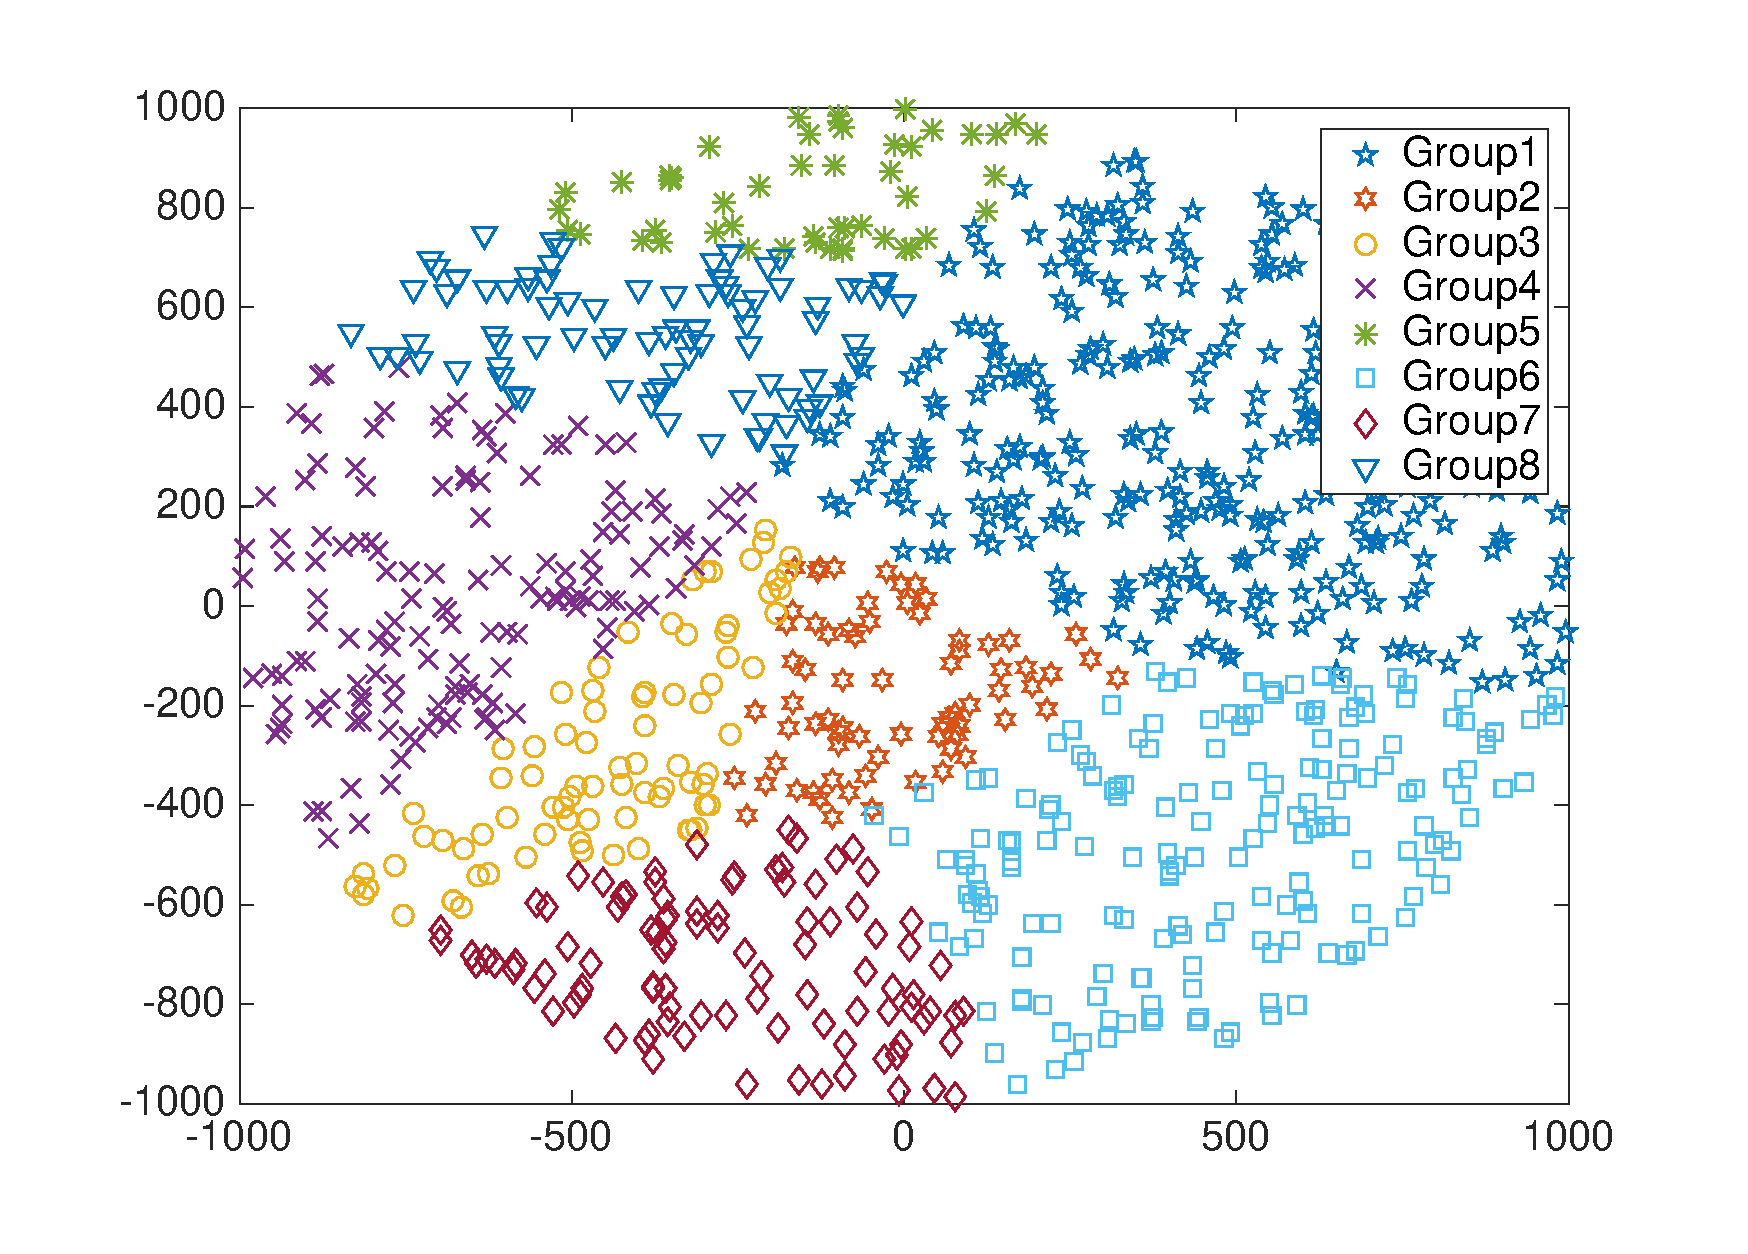
\includegraphics[width=.95\textwidth]{figures/sample_vonoroli}
  \caption{A sample grouping showing how nodes are categorized location-wise using RSS-based grouping}
  \label{fig:samplevonoroli}
\end{figure}


\subsection{Implementation Issues}
The proposed scheme can be readily implemented in current IEEE 802.11 systems without any major modifications. The power measurement already exists in the MAC layer of all systems and they can provide RSSI at any time, so nodes can then find the sensed power of each GST transmission by measuring the average RSSI during the reception time of the pilot. 

GST can be as small as an ACK time and there should be some guard distance time between pilot transmissions from group heads. For the best performance, the optimum value of GUP and GST should be determined which is beyond the scope of this paper and they do not affect our following analysis. The grouping can also be triggered by the AP if the randomly selected headers result in unsatisfactory network performance.

Including $M$ in BF is something that is already being done in the IEEE standard draft \cite{Draft80211ah}. Informing group heads about their index can also be done using a mapping strategy similar to the one used for delivery traffic indication known as DTIM.

Our algorithm is also robust against interference from other APs. Since the GSTs are short and they could be transmitted consecutively with a gap of SIFS, any other CSMA/CA based station, e.g. other APs, cannot transmit anything during the grouping procedure.

\subsection{Analytical Model}

In order to compare the performance of grouping schemes on hidden-terminal probability, here we define two metrics and use them along with the probability of having a hidden terminal in a group to show the benefits and costs of each grouping scheme. The first metric is the average distance between nodes in a group, $D_m$, which is defined as
\begin{equation}
D_m=\frac{\sum_{i} \sum_{j \neq i} d_{ij}}{{n_m \choose 2}},  \quad \quad \forall i \text{ and } j \in \text{group $m$},
\end{equation}
where $n_m$ is the number of nodes in group $m$ and $d_{ij}$ is the distance between nodes $i$ and $j$.

The second metric is the standard deviation of the number of nodes in different groups which specifies how evenly nodes are distributed between different groups.
\begin{equation}
\sigma=\sqrt{\frac{1}{M}\sum_{m=0}^{M-1}\left( n_m - \frac{N}{M} \right)^2},
\end{equation}
where $N$ is the total number of nodes and $M$ is the number of available groups.

The next step is finding the probability of encountering the hidden terminal problem for different schemes. The number of group head nodes in our proposed strategy is fixed so their locations follow Binomial Point Process (BPP) and there are $M$ of them in the entire coverage area. Thus, the probability that there are $k$ group heads in an area of size $B$ can be found as
\begin{equation}
Pr[ N(B)=k | N(A)=M]={M \choose k} \left( \frac{B}{A} \right)^k \left( 1- \frac{B}{A} \right)^{M-k},
\end{equation}
where $A=\pi R^2$ is total area of network. We use $D$ to denote the distance between one node and its nearest group head. Every node will find its nearest group head, therefore for the CDF of $D$ we have
\begin{equation}
F_D(x)=1-Pr[N(S(x))=0 | N(A)=M] \quad x \geq 0,
\end{equation}
where $S(x)$ is the overlapping area between a circle centered at the observed node with radius $x$ and the coverage area. In general $S(x) \leq \pi x^2$ and the inequality happens for nodes close to the coverage area's border. We define $\hat{F_D(x)}$ by
\begin{equation}
\hat{F_D(x)}=1-Pr[N(\pi x^2)=0 | N(A)=M] \quad 0 \leq x \leq R.
\end{equation}
It is always true that $\hat{F_D(x)} \geq F_D(x)$ for $0 \leq x \leq R$. However, when M is large enough, which is typically the case in practice \cite{zheng2014performance} the group size is so small comparing with the whole network area that the difference between $F_D(x)$ and $\hat{F_D(x)}$ becomes negligible. We use the latter as an upper-bound of the real case.
\begin{equation} \label{eq:cdf}
\begin{split}
F_D(x) \approx \hat{F_D(x)} &=1-Pr[N(\pi x^2)=0 | N(A)=M] \\
&=1- {M \choose 0} \left( \frac{\pi x^2}{A} \right)^0 \left( 1- \frac{\pi x^2}{A} \right)^{M} \\
&=1- \left( 1- \frac{\pi x^2}{A} \right)^{M} \quad 0 \leq x \leq R.
\end{split}
\end{equation}
%The probability that $x \geq R$ is neglected in the above CDF because it is very low.
The validity of this approximation is then verified by simulation in Section \ref{evaluation}.

We can find PDF of $D$ by taking derivative of its CDF:
\begin{equation} \label{eq:pdf}
f_D(x)=\frac{2\pi M x}{A}(1-\frac{\pi x^2}{A})^{M-1} \quad 0 \leq x \leq R.
\end{equation}
Using this PDF we can find the probability of having a hidden terminal when our RSS-based grouping scheme is used.
\begin{figure}[h]
    \centering
    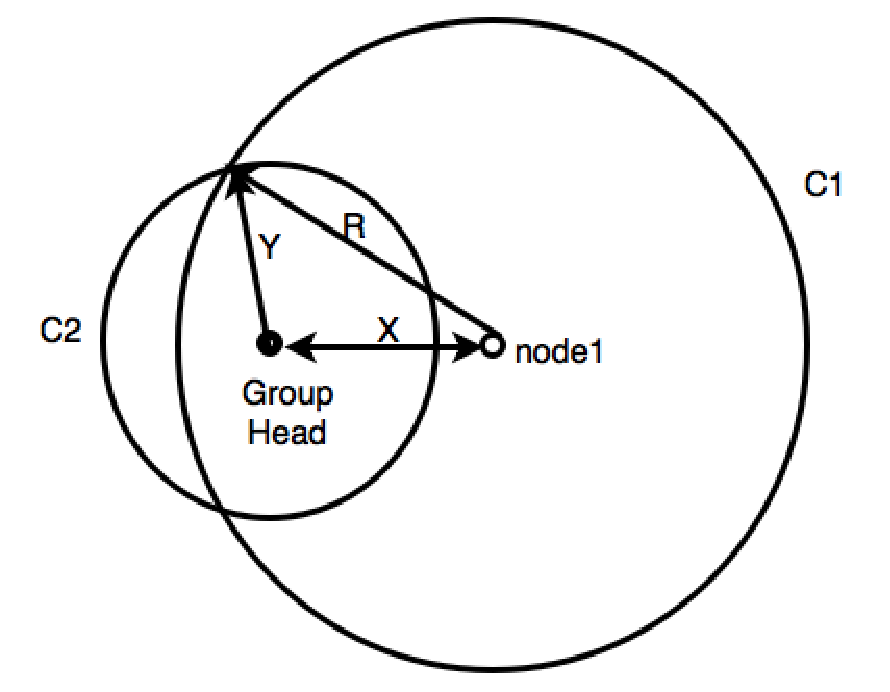
\includegraphics[width=0.75\textwidth]{figures/webb2}
    \caption{Two nodes and group head in one Voronoi cell}
    \label{fig:geometrit}
\end{figure}

Figure \ref{fig:geometrit} shows a group head and a random node called node 1 in the same group in distance $X$ where $X$ follows the PDF in (\ref{eq:pdf}). \iffalse The other node is assumed to be anywhere Within Y distance of group head. \fi The circle C1 shows the sensing range of node 1 and C2 is a circle centered by the group head with the raduis Y which also follows the PDF in (\ref{eq:pdf}). The probability for node 2 which is Y away from the group head to be in the sensing range of node 1 is the ratio of the portion of C2 inside C1 to the perimeter of C2. Then, we can take the average over the PDF of $X$ and $Y$ to obtain the probability that two nodes are within each other's sensing range.

\begin{equation}
\begin{split}
Pr_{\text{sense}}=& \\
& \int_0^{\sqrt{\frac{A}{\pi}}}\int_0^{\sqrt{\frac{A}{\pi}}} \frac{g_1(x,y)}{2\pi y} f_X(x) f_Y(y) dxdy,
\end{split}
\end{equation}
where $Pr_{\text{sense}}$ is the probability that two nodes in the same group are in each other's sensing range, $R_s$ is the sensing range of a node, 
\begin{equation}
g_1(x,y)=
\begin{cases} 
      2\pi y & R_s\geq x+y \\
      2y\arccos(\frac{x^2+y^2-R_s^2}{2xy}) & R_s< x+y \\
      0 & R_s < |x-y| 
   \end{cases},
\end{equation}
and $f_X(x)$ and $f_Y(y)$ are the PDF of $X$ and $Y$ respectively. 

We can also derive the same probability for random grouping schemes. The probability density function for the distance between two random nodes in a circle with the radius $R$ is given in \cite{moltchanov2012distance}
\begin{equation}
\begin{split}
f(r)=\frac{2r}{R^2} & \left( \frac{2}{\pi}\arccos(\frac{r}{2R}) \right. \\
& \left.  - \frac{r}{\pi R} \sqrt{1- \frac{r^2}{4R^2}} \right ) ,\quad 0<r<2R.
\end{split}
\end{equation}
In this case, for random grouping, the probability of that two nodes in the same group are in each other's sensing region can be obtained as follows,
\begin{equation}
Pr_{\text{sense}}=\int_0^{2R}g_2(r)f(r)dr,
\end{equation}
where
\begin{equation}
g_2(r)=
\begin{cases} 
      1 & r \leq R_s \\
      0 & r > R_s
   \end{cases}.
\end{equation}
These probabilities can then be calculated by numerical methods.